\chapter{Programsko ostvarenje protokola ACAP}
\label{ch:impl}

Programsko ostvarenje ACAP izvedeno je u programskom jeziku Python 3 koji
koristi dodatne biblioteke za kriptografiju
(pycrypto\footnote{https://www.dlitz.net/software/pycrypto/} i
cryptography\footnote{https://cryptography.io/en/latest/}) i biblioteku za
prepoznavanje mrežnih sučelja za
potrebe rada na sloju Ethernet
(netifaces\footnote{https://pypi.python.org/pypi/netifaces}). Programsko
ostvarenje podržava
pokretanje aplikacije u klijentskom i poslužiteljskom načinu rada i kao rezultat
vraća sljedeće podatke:
\begin{itemize}
\item popis dogovorenih algoritama razvrstanih u kategorije,
\item tajni ključ koji se može koristiti za osiguravanje tajnosti korištenjem
simetričnih algoritama šifriranja i dešifriranja ili osiguravanje
cjelovitosti korištenjem algoritma HMAC i
\item javni ključ druge strane koji se može koristiti za provjeru identiteta i
osiguravanje cjelovitosti korištenjem digitalnog potpisa.
\end{itemize}

U ovom poglavlju objašnjen je način rada ostvarenja protokola
ACAP kroz pokretanje na različitim mrežnim slojevima i prikaz strukture poruka.
Nakon toga dana je analiza performansi uz mjerenja koja prikazuju složenost
kriptografskih operacija. Na kraju poglavlja prikazani su ugrađeni sigurnosni
mehanizmi. Aktualna verzija programskog ostvarenja uz upute za instalaciju može se
dohvatiti sa sljedeće poveznice:
\begin{center}
    \url{http://public.tel.fer.hr/acap}
\end{center}

\section{Arhitektura programskog ostvarenja i načini integracije}
Protokol ACAP sastoji se od sljedećih sastavnih dijelova:
\begin{itemize}
    \item izračun i provjera kriptografskih algoritama,
    \item obrada poruka,
    \item komunikacija neovisna o sloju,
    \item dogovor kriptografskih algoritama i
    \item komunikacija s vanjskim aplikacijama.
\end{itemize}

Cjelokupna arhitektura programskog ostvarenja prikazana je na slici \ref{fig:impl}.
Nakon što protokol ACAP zaprimi zahtjev za dogovorom kriptografskih algoritama
kroz sustav za komunikaciju s vanjskim aplikacijama, pokreće se proces dogovora
algoritama i ključeva prema ACAP poslužitelju na drugoj strani. U dogovoru se
međusobno izmjenjuju sustavi za izračun i provjeru kriptografskih algoritama,
obradu poruka te slanje i primanje paketa. Na kraju dogovora
pokreće se sustav za dogovor algoritma koji daje popis dogovorenih algoritama,
na temelju kojih se generira dogovorena duljina kriptografskog ključa uz pomoć
funkcije za generiranje nasumičnih vrijednosti. Na kraju
se popis dogovorenih algoritama zajedno s kriptografskim ključevima šalje
aplikaciji koja je pokrenula dogovor. Nakon ACAP razmjene pozivajuća aplikacija
može sigurno komunicirati korištenjem dogovorenih algoritama i ključeva.

\begin{figure}[htb]
    \centering
    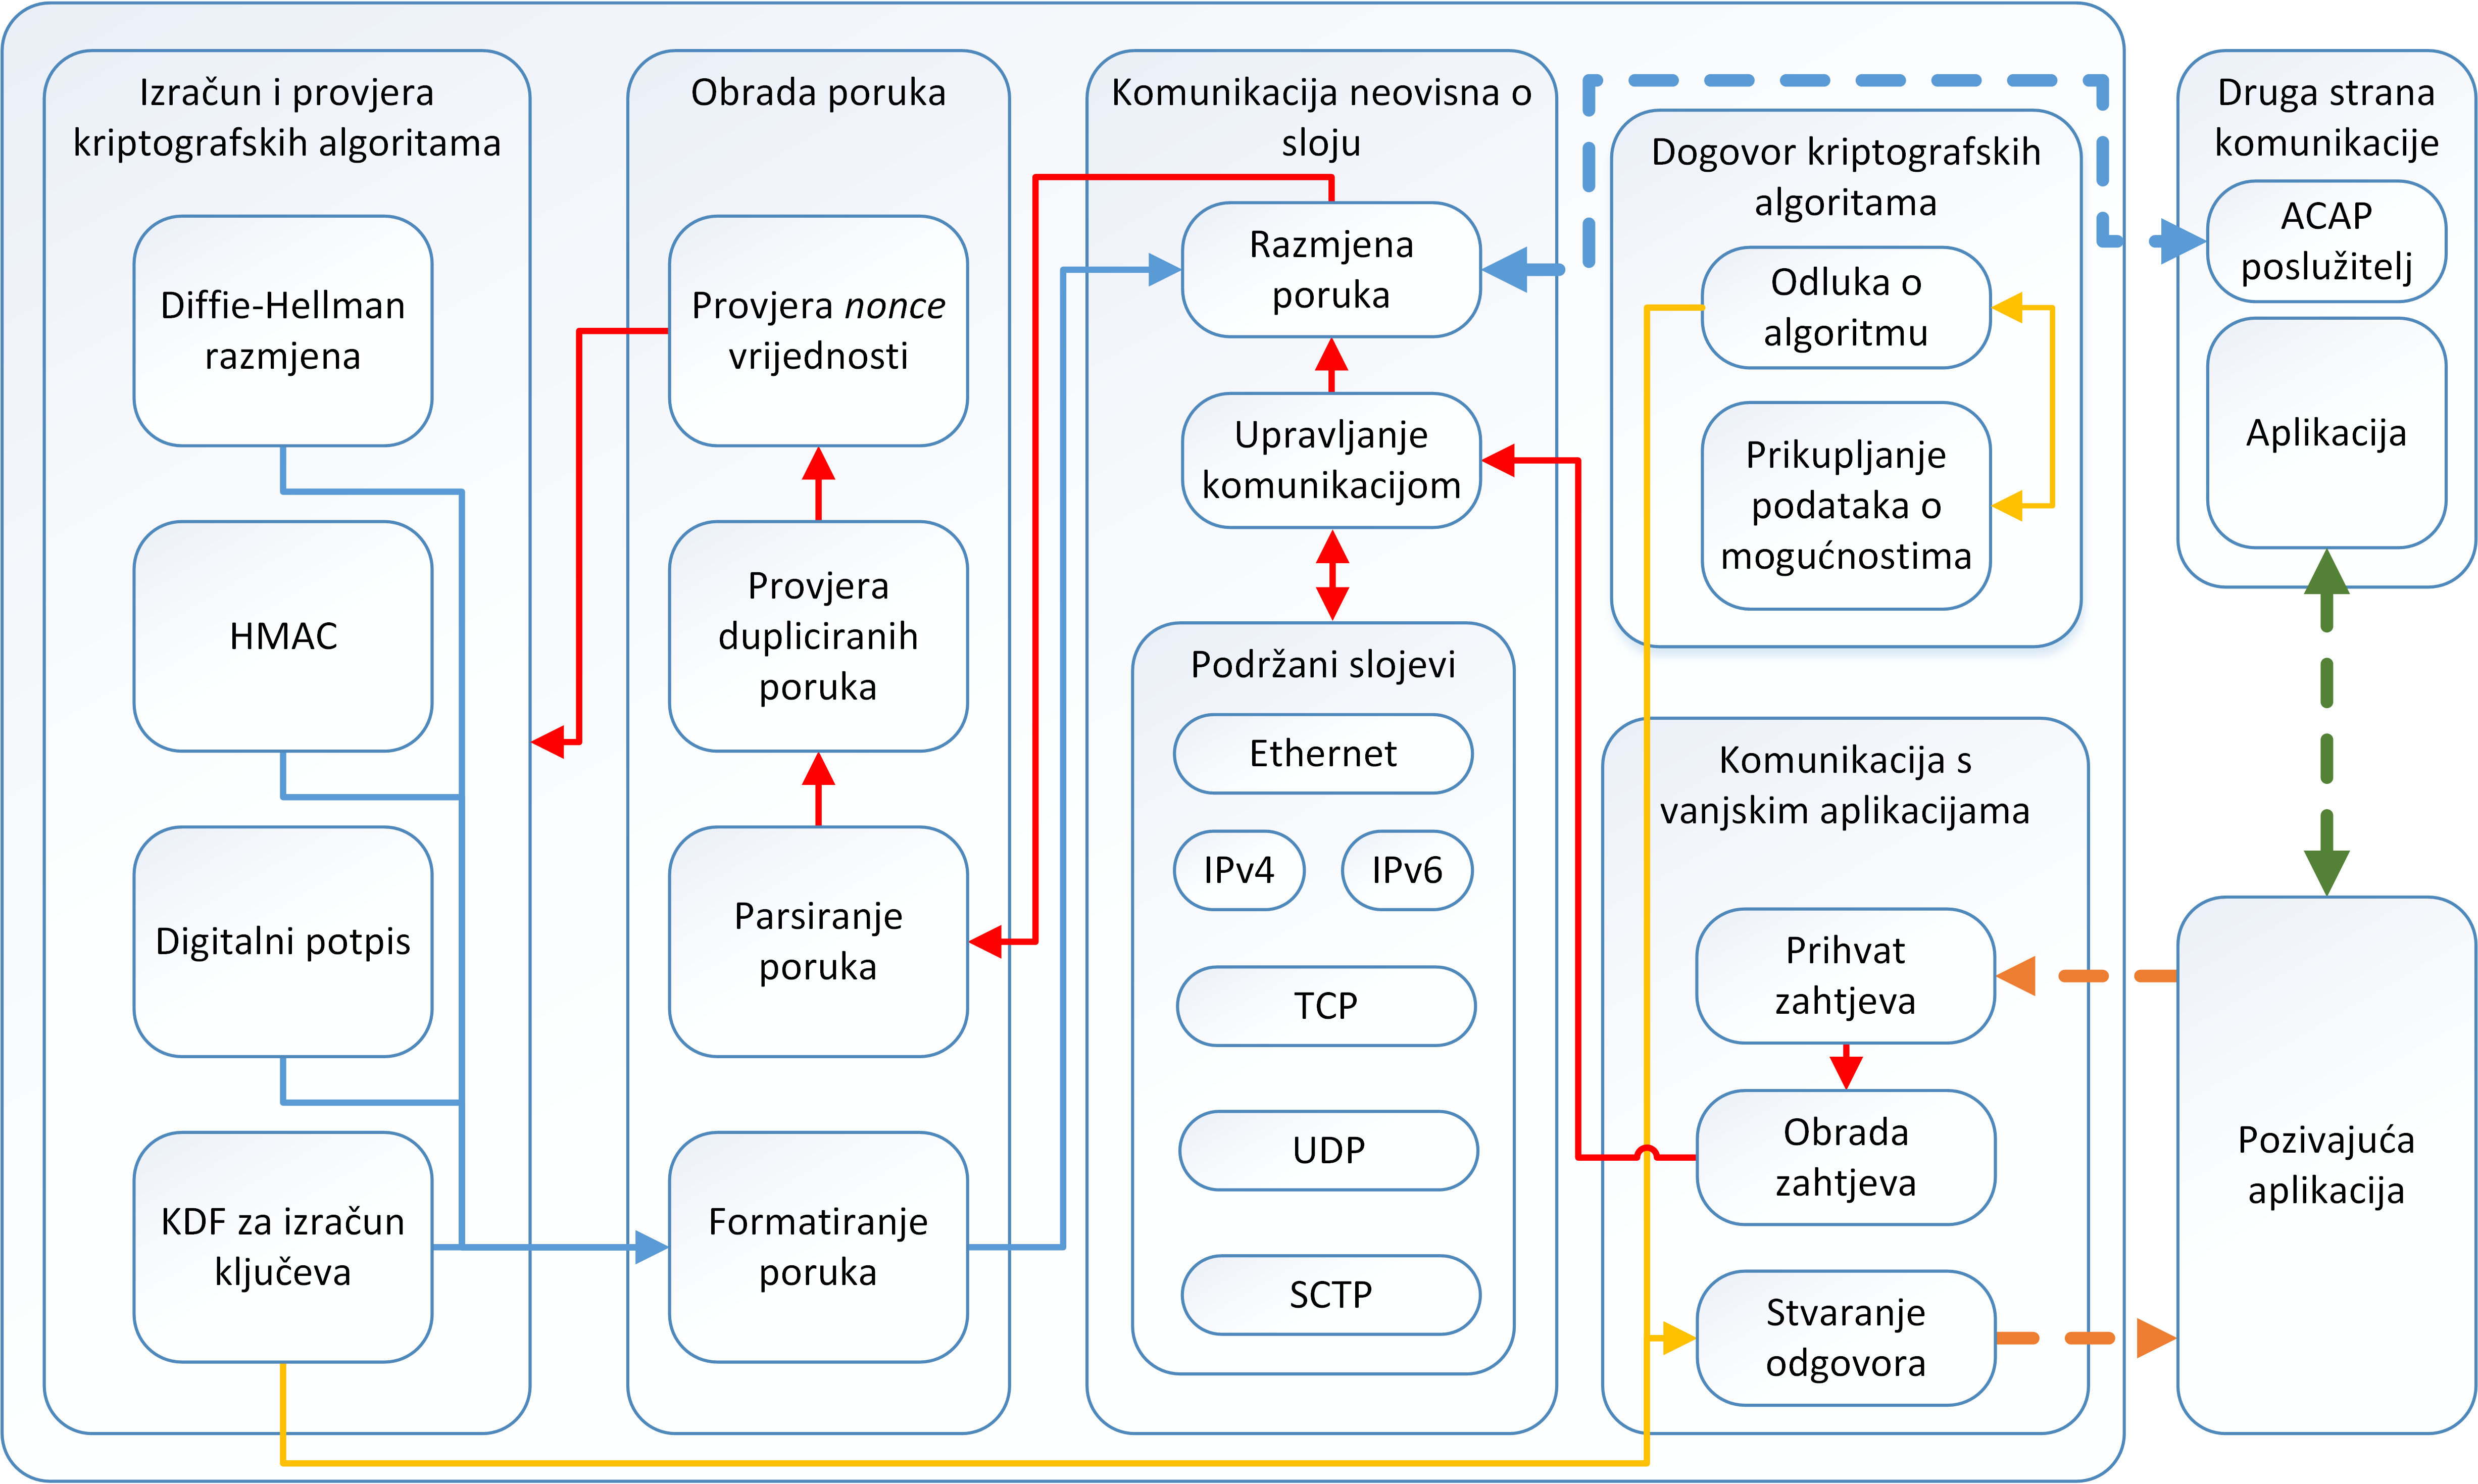
\includegraphics[width=0.98\textwidth]{arhitektura}
    \caption{Arhitektura programskog ostvarenja protokola ACAP}
    \label{fig:impl}
\end{figure}

Programsko ostvarenje protokola ACAP izravno podržava primjenu u sklopu modela
klijent-poslužitelj.
Primjena u mrežama ravnopravnih čvorova
postiže se pokretanjem poslužitelja na svim čvorovima u mreži te se dogovor
algoritama i ključeva odvija u parovima čvorova. Na taj način omogućeno je da
komunikacija između svaka dva čvora u mreži dobije razinu zaštite komunikacije
koja je primjerena mogućnostima tih čvorova. Grupni dogovor ključeva i
algoritama između ravnopravnih čvorova nije omogućen jer bi to nužno smanjivalo
razinu sigurnosti na mogućnosti najslabijeg čvora i omogućilo napadaču
razne napade na sigurnost samog protokola.

\section{Mogućnosti programskog ostvarenja}
Prilikom pokretanja ostvarenja moguće je specificirati hoće li se pokrenuti
poslužiteljska ili klijentska instanca protokola. U slučaju klijentske strane
potrebno je definirati adresu poslužitelja. Nadalje, može se specificirati koji
se protokol želi koristiti za prijenos poruka. Moguće je odabrati između
protokola TCP, SCTP, UDP, IP i Ethernet. Dodatno, za protokole TCP,
SCTP, UDP i IP moguće je koristiti protokol IP verzije 4 i protokol IP verzije 6.
Pretpostavljene opcije prilikom pokretanja su korištenje protokola TCP s IPv4
adresama za transport, korištenje standardnog Diffie-Hellman postupka i
algoritma RSA za digitalno potpisivanje.

Za osnovno pokretanje potrebno je definirati želi li se pokrenuti poslužitelj
ili klijent. Za pokretanje poslužitelja koristi se opcija "\texttt{-S}", a za
pokretanje klijenta opcija "\texttt{-C}". Potrebno je definirati popis podržanih
algoritama s opcijom "\texttt{-a}", u suprotnom će se popis algoritama
automatski dohvatiti iz trenutno dostupnih kriptografskih algoritama u sustavu.
Nužno je još definirati privatni ključ s pomoću opcije "\texttt{-k}", koja uzima
datoteku s RSA privatnim ključem veličine barem 768 okteta. Iz tog
privatnog ključa dobiva se javni ključ koji služi za identifikaciju tijekom
razmjene. Rezultati uspješne razmjene prikazani su na slikama
\ref{fig:acap_client} i \ref{fig:acap_server}.

Na slici \ref{fig:acap_client} vidi se skraćeni ispis pokretanja klijenta kojemu
je potrebno dodatno definirati adresu poslužitelja na koju će se spojiti
("\texttt{-h 10.0.0.20}"). Nakon
razmjene poruka klijent dobiva javni ključ poslužitelja, popis
dogovorenih algoritama i dijeljenu zajedničku tajnu. Na kraju ispisa prikazano
je ukupno trajanje dogovora od početka razmjene. Potpuni ispis klijenta sa svim
ključevima moguće je vidjeti u dodatku \ref{app:cli_impl}.

\begin{figure}[htb]
\begin{footnotesize}
\begin{verbatim}
$ ./acap.py -C -a client.json -k private_key_client -h 10.0.0.20
INFO - Server public key: -----BEGIN PUBLIC KEY-----
MIGfMA0GCSqGSIb3DQEBAQUAA4GNADCBiQKBgQCTYB3xU17CS5AGxKbWraxuGOYb
7sff8AAjjiwXrdBr6jqJ5zSHtR/bKxsRNPMNvzihVI1Taa7/CQy3EIRKkLeG4I7M
USeStpBfvQlpAK+lmyUE3haXVUNgPpALdXUpn+IaB+TDHuWl19z9dPDkSDLzQzga
pVwSgXpEZDUInwKK4QIDAQAB  -----END PUBLIC KEY-----
INFO - Client negotiated: 
{  "hash": {
        "algorithm": "SHA-256",
        "timestamp": "2015-11-22 14:59" },
    "public_key": {
        "algorithm": "RSA_2048",
        "timestamp": "2015-11-22 14:59" },
    "secret_key": {
        "algorithm": "AES-CTR_256",
        "timestamp": "2015-11-22 14:59" } }
INFO - Shared secret key (256 bit): bb:66:cc:98:10:fd:b7:a0:73:9b:9e:35:49:11:
43:7e:e5:28:3d:b3:69:5e:e2:69:4c:c9:a8:11:6d:d5:57:9a
INFO - TOTAL duration: 119820
\end{verbatim}
\end{footnotesize}
\vspace{-15pt}
\caption{Primjer pokretanja ACAP klijenta}
\label{fig:acap_client}
\end{figure}

Na slici \ref{fig:acap_server} prikazan je skraćeni ispis sa strane
poslužitelja.
Jedina značajna razlika vidljiva je u prvoj liniji koja označava da
su osvježene vrijednosti Diffie-Hellman eksponenta i poslužiteljski \emph{nonce}
("\texttt{Refreshed DH and Nonce...}"). Taj se proces kod poslužitelja odvija u
pozadini i služi za smanjenje utjecaja DoS napada na protokol ACAP na način
opisan u poglavlju \ref{sec:sigurnost}. Potpuni prikaz poslužitelja sa svim
ključevima prikazan je u dodatku \ref{app:serv_impl}.

\begin{figure}[htb]
\begin{footnotesize}
\begin{verbatim}
$ ./acap.py -S -a server.json -k private_key_server
Refreshed DH and Nonce...
INFO - Client public key: -----BEGIN PUBLIC KEY-----
MIGfMA0GCSqGSIb3DQEBAQUAA4GNADCBiQKBgQC4TDSclGnCkXgP0C8mt889rBRl
iFoXBtOlG4VF1XxhxursgU+Es2PCqRUYT28ZqdNrq2CAyuIT33G5CXCwg8x/CBh2
qmFJ43NpauGg13b2LFNSg3j8UxxwGSGIvKvxOmaGnSJByepogXkWuY0bL5mR0n0l
JPH/imO5V2+Jox951QIDAQAB  -----END PUBLIC KEY-----
INFO - Server negotiated: 
{   "hash": {
        "algorithm": "SHA-256",
        "timestamp": "2015-11-22 14:59" },
    "public_key": {
        "algorithm": "RSA_2048",
        "timestamp": "2015-11-22 14:59" },
    "secret_key": {
        "algorithm": "AES-CTR_256",
        "timestamp": "2015-11-22 14:59" } }
INFO - Shared secret key (256 bit): bb:66:cc:98:10:fd:b7:a0:73:9b:9e:35:49:11
:43:7e:e5:28:3d:b3:69:5e:e2:69:4c:c9:a8:11:6d:d5:57:9a
INFO - TOTAL duration: 17757
\end{verbatim}
\end{footnotesize}
\vspace{-15pt}
\caption{Primjer pokretanja ACAP poslužitelja}
\label{fig:acap_server}
\end{figure}

Prilikom pokretanja moguće je odabrati kriptografske algoritme koji se
zasnivaju na korištenju eliptičkih krivulja. To se radi s pomoću opcije
"\texttt{-E}" koja specificira da se umjesto standardnog Diffie-Hellman postupka
koristi ECDH (engl. \emph{Elliptic Curve Diffie-Hellman}) te da se umjesto
algoritma RSA koristi algoritam ECDSA za digitalno potpisivanje. Tada se
umjesto privatnog RSA ključa mora specificirati ECDSA privatni ključ.

\comment{lokalna baza s rezultatom dogovora, prvo implementirati, pa onda prikazati}

\section{Struktura poruka}

Poruke koje se razmjenjuju u protokolu ACAP prikazane su u poglavlju
\ref{sec:poruke}. S obzirom na to da su osnovni dijelovi tih poruka varijabilne
duljine, prije svakog od tih dijelova dodano je polje koje označava duljinu
parametra. Bitovni zapis poruke \initi{} prikazan je na slici \ref{fig:initi_fmt}. Za
definiranje svih duljina koriste se dva okteta koja sadrže duljinu polja
izraženu u broju okteta. Formati ostalih poruka nalaze se u dodatku
\ref{app:formats}.

\begin{figure}[htb]
    \centering
\begin{bytefield}[bitwidth=0.75em]{32}
\bitheader{0,7,15,23,31} \\
\bitbox{16}{\colorbox{blue!30}{Duljina poruke}} & \bitbox{8}{\colorbox{red!30}{Tip=0}} & \bitbox{8}{\colorbox{yellow!30}{Duljina DH}} \\
\bitbox{8}{\colorbox{yellow!30}{Duljina DH}} & \bitbox[lr]{24}{} \\
\wordbox[lr]{2}{\colorbox{orange!30}{Klijentov Diffie-Hellman javni dio} \\ $\vdots$} \\
\bitbox{16}{\colorbox{green!30}{Duljina \emph{noncea}}} & \bitbox[lrt]{16}{} \\
\wordbox[lrb]{2}{\colorbox{purple!30}{Klijentov \emph{nonce}} \\ $\vdots$}
\end{bytefield}
\caption{Bitovni zapis poruke \initi{}}
\label{fig:initi_fmt}
\end{figure}

Na slici \ref{fig:initi_bits} dan je bitovni prikaz jedne poruke \initi{} koji je
obojan u skladu s bitovnim zapisom iz slike \ref{fig:initi_fmt} kako bi se lakše
identificirala polja poruke. Na početku se nalazi duljina poruke u oktetima
(\texttt{0x0091}=145), potom je naveden tip poruke (\texttt{0x00}), a zatim
duljina DH javnog dijela klijenta (\texttt{0x0080}=128) i vrijednost DH javnog
dijela. Na samom kraju poruke
zapisana je duljina klijentovog \emph{noncea} (\texttt{0x000c}=12) i vrijednost
\emph{noncea}.
Cjelokupna duljina poruke jednaka je zbroju duljina svih navedenih dijelova
($1+2+128+2+12=145$).

\begin{figure}[htb]
\begin{center}
\begin{minipage}{0.6\linewidth}
\begin{footnotesize}
\begin{monoblock}
\noindent 0x00:\colorbox{blue!30}{00 91}\colorbox{red!30}{00}\colorbox{yellow!30}{00 80}\colorbox{orange!30}{27 2d d0 e9 6a f9 d7 37 2e a1 c8} \\
0x10:\colorbox{orange!30}{6c 23 0a c9 44 98 13 c6 ed 27 fc ac b8 3c 91 dc} \\
0x20:\colorbox{orange!30}{82 4a 1d f0 af 47 5a 87 63 42 24 0b e4 2b e1 0f} \\
0x30:\colorbox{orange!30}{e0 1f fa 54 c6 14 5d 4f bf 13 c6 76 70 5f 65 06} \\
0x40:\colorbox{orange!30}{8d 74 c6 1f 9f 1f 00 dd 71 55 65 d3 09 44 da 59} \\
0x50:\colorbox{orange!30}{cf 37 74 e1 f1 b3 38 55 38 51 20 b9 25 c8 68 b0} \\
0x60:\colorbox{orange!30}{03 cd e0 dd 97 34 ab 99 3e 75 36 c2 8f 78 fd b9} \\
0x70:\colorbox{orange!30}{9e a5 7e df bc ee ea 50 d0 f0 8e ce 4d 02 e8 75} \\
0x80:\colorbox{orange!30}{b5 9b 5e 62 d7}\colorbox{green!30}{00 0c}\colorbox{purple!30}{c7 48 6b 13 6f d8 16 e0 00} \\
0x90:\colorbox{purple!30}{15 ce 6b}
\end{monoblock}
\end{footnotesize}
\end{minipage}
\vspace{-20pt}
\end{center}
\caption{Bitovni prikaz primjera poruke \initi{}}
\label{fig:initi_bits}
\end{figure}

Formati poruka i njihov bitovni zapis u potpunosti je neovisan o transportnom
protokolu. Transportni protokol određuje isključivo kako će se popunjavati
zaglavlja i na koji će se način protokol ACAP razlikovati da bi se mogao
obrađivati neovisno o drugom prometu.

\section{Korištenje protokola na različitim komunikacijskim slojevima}

Kako bi se mogli koristiti različiti komunikacijski protokoli za prijenos
podataka uvedeni su posebni mehanizmi. Ti se mehanizmi dijele u dvije osnovne
skupine: mehanizmi kod pouzdanog prijenosa podataka i mehanizmi kod nepouzdanog
prijenosa podataka.

Pouzdani prijenos podataka obuhvaća prije svega protokol TCP~\cite{rfc793}. S
obzirom na to da protokol TCP za prijenos koristi tokove podataka, a protokol ACAP
komunikaciju porukama, svakoj poruci potrebno je dodati duljinu poruke
kako bi se mogla izdvojiti iz toka podataka.

Nepouzdani prijenos podataka odnosi se na prijenos s pomoću protokola
UDP~\cite{rfc768}, IPv4~\cite{rfc791}, IPv6~\cite{rfc2460} Ethernet (IEEE 802.3)
i sličnim. Prijenos s
pomoću tih protokola odvija se porukama. Kako se radi o nepouzdanom prijenosu,
potrebno je detektirati gubitak poruka i obaviti ponovno slanje poruke u slučaju
gubitka. Taj problem se rješava na sličan način kao kod protokola
DTLS~\cite{rfc6347}, korištenjem brojila (\emph{expire timer}). Brojilo počinje
odbrojavati nakon što se pošalje poruka. Ako brojilo odbroji do kraja i ne primi
povratnu poruku, ponovno šalje istu poruku. Ako se poruka izgubi tri puta
uzastopno, dogovor se prekida. Uz to, potrebno je riješiti problem dupliciranja
datagrama na putu do odredišta. To se rješava prepoznavanjem kopija poruka i
njihovim odbacivanjem u okviru određenog vremenskog prozora. Za svaku dolaznu
poruku računa se kriptografski sažetak i uspoređuje se sa sažecima prijašnjih
poruka. Ako sažetak postoji u privremenoj bazi sažetaka poruka se odbacuje, a u
suprotnom se sažetak poruke sprema u privremenu bazu sažetaka.

Kod korištenja datagramskog prijenosa podataka potrebno je obratiti pozornost na
to da poruka svojom veličinom ne prijeđe veličinu određenu najmanjom vrijednošću
MTU-a (\emph{Maximum Transmission Unit}) na putu do odredišta~\cite{rfc1191}.
Kod korištenja protokola UDP i IP to je nužno da bi se spriječila fragmentacija
datagrama u više paketa što bi povećalo mogućnost gubitka paketa. Protokolom
ACAP moguće je poslati pakete proizvoljne veličine, ali u slučaju korištenja
protokola Ethernet kao transportnog protokola, najveća veličina okvira može biti
1500 okteta, kako bi se izbjegla nekompatibilnost s postojećim mrežama.

\subsection{Protokol Ethernet}
Komunikacija na sloju podatkovne poveznice protokolom Ethernet specificira se
korištenjem opcije "\texttt{-e}" uz specifikaciju mrežnog sučelja preko kojeg se
želi komunicirati. Primjeri poziva za klijenta i poslužitelja:
\begin{footnotesize}
\begin{verbatim}
# ./acap.py -C -a client.json -k private_key_client -e eth0 -h 00:01:29:f0:83:a4
# ./acap.py -S -a server.json -k private_key_server -e eth0
\end{verbatim}
\end{footnotesize}

Ethernet zaglavlje za slanje poruke \initi{} bit će definirano na sljedeći
način: \\
\begin{footnotesize}
\begin{monoblock}
\noindent 0x00:\colorbox{blue!30}{00 01 29 f0 83 a4}\colorbox{yellow!30}{74 d0 2b 93 24 f8}\colorbox{orange!30}{08 13}
\end{monoblock}
\end{footnotesize}

Prve dvije vrijednosti označavaju redom MAC adrese poslužitelja i
klijenta, a zadnja vrijednost specificira identifikator protokola ACAP
(\texttt{0x0813}) na Ethernet sloju. Podaci koje prenosi Protokol Ethernet za
poruku \initi{} formatirani su kao na slici \ref{fig:initi_fmt}.

\subsection{Protokoli IP}
Ako se podaci u sklopu razmjene poruka prenose protokolom IP ili višim, moguće je
odabrati želi li se koristiti protokol IPv4 ili IPv6. Pretpostavljena opcija je
korištenje protokola IPv4 ("\texttt{-4}"), a korištenje protokola IPv6 definira
se korištenjem opcije "\texttt{-6}". Primjeri poziva za
klijenta i za poslužitelja za protokol IPv4:
\begin{footnotesize}
\begin{verbatim}
# ./acap.py -C -a client.json -k private_key_client -i 10.0.0.21
# ./acap.py -S -a server.json -k private_key_server -i
\end{verbatim}
\end{footnotesize}

IPv4 zaglavlje za slanje početne poruke definirano je na sljedeći način:
\begin{figure}[H]
\begin{footnotesize}
\begin{monoblock}
\noindent 0x00:\colorbox{blue!30}{4}5 00 00 a7 d6 8d 40 00 40\colorbox{yellow!30}{b7}4e ea\colorbox{orange!30}{0a 00 00 14} \\
0x10:\colorbox{purple!30}{0a 00 00 15}
\end{monoblock}
\end{footnotesize}
\vspace{-10pt}
\end{figure}

Prva naznačena vrijednost predstavlja verziju protokola IP (\texttt{4}), a druga
vrijednost je identifikator protokola ACAP kojeg prenosi protokol IPv4
(\texttt{0xb7}=183). Posljednje dvije vrijednosti su IP adrese klijenta
(\texttt{0x0a 0x00 0x00 0x14=10.0.0.20}) i poslužitelja (\texttt{0x0a 0x00 0x00
0x15=10.0.0.21}).

Primjeri poziva za klijenta i poslužitelja za protokol IPv6:
\begin{footnotesize}
\begin{verbatim}
# ./acap.py -C -a client.json -k private_key_client -6 -i -h fc00::21
# ./acap.py -S -a server.json -k private_key_server -6 -i
\end{verbatim}
\end{footnotesize}

Za dani primjer poziva IPv6 zaglavlje će biti sljedeće:

\begin{figure}[H]
\begin{footnotesize}
\begin{monoblock}
\noindent 0x00:\colorbox{blue!30}{6}0 00 00 00 00 93\colorbox{yellow!30}{b7} 40\colorbox{orange!30}{fc 00 00 00 00 00 00 00} \\
0x10:\colorbox{orange!30}{00 00 00 00 00 00 00 20}\colorbox{purple!30}{fc 00 00 00 00 00 00 00} \\
0x20:\colorbox{purple!30}{00 00 00 00 00 00 00 21}
\end{monoblock}
\end{footnotesize}
\vspace{-10pt}
\end{figure}

Prva obojana vrijednost je verzija protokola IP (\texttt{6}), a druga vrijednost
je identifikator protokola ACAP (\texttt{0xb7}=183). Posljednje dvije
vrijednosti su IP adrese klijenta (\texttt{fc00::20}) i poslužitelja
(\texttt{fc00::21}).

\subsection{Transportni protokoli}

U programskom ostvarenju trenutno su podržana tri transportna protokola: TCP, UDP i
SCTP. Kod sva tri protokola poslužitelji slušaju na vratima 13000 za dogovor
putem protokola ACAP.
Pretpostavljena vrijednost je korištenje protokola TCP ("\texttt{-t}").
Korištenje protokola UDP definira se opcijom "\texttt{-u}", a korištenje
protokola SCTP opcijom "\texttt{-s}". Definiranje adrese klijenta ovisi o tome
koristi li se protokol IPv4 ili IPv6.

Za cjelokupnu razmjenu protokolu TCP potrebno je 12 IP paketa, protokolu UDP 4
paketa, a protokolu SCTP 13 paketa. Zbog početnih kontrolnih poruka koje su
nužne za uspostavu veze kod protokola TCP i SCTP te  veće složenosti zaglavlja
prikazano je samo zaglavlje prilikom korištenja protokola UDP. Zaglavlje kod
korištenja protokola UDP za prvu poruku je sljedeće:
\begin{figure}[h]
\begin{footnotesize}
\begin{monoblock}
\noindent 0x00:\colorbox{blue!30}{b8 d2}\colorbox{yellow!30}{32 c8}00 9b fe ae
\end{monoblock}
\end{footnotesize}
\vspace{-10pt}
\end{figure}

Prva obojana vrijednost označava odlazna vrata koja se automatski dodjeljuju od
strane operacijskog sustava (\texttt{0xb8d2}=47314), a druga vrijednost označava
vrata na kojima sluša ACAP poslužitelj (\texttt{0x32c8}=13000).

\section{Mjerenje performansi protokola u emuliranoj mrežnoj okolini}

Mjerenje performansi protokola izvedeno je u emuliranoj mrežnoj okolini IMUNES.
Emulirana mrežna okolina predstavlja mrežnu okolinu koja se izvodi na jednom ili
više računala u stvarnom vremenu i uz standardan način obrade paketa.
IMUNES\footnote{http://www.imunes.net} je
mrežni emulator koji može na vrlo efikasan način izvršavati emulirane mrežne
okoline od 100 i više mrežnih uređaja na jednom računalu
\cite{salopek2014network}. Paketi se u
IMUNES emuliranoj mrežnoj okolini obrađuju na način na koji je to definirano u
sklopu FreeBSD ili Linux jezgre operacijskog sustava. U toj emuliranoj
mrežnoj okolini moguće je definirati razne smetnje na poveznicama između čvorova
kako bi se lakše ispitala robusnost programskog ostvarenja.

Za potrebe testiranja i mjerenja protokola ACAP koristi se jednostavna emulirana
mrežna topologija koja je prikazana na slici \ref{fig:imunes}. Topologija se
sastoji od dva čvora, jedan za klijenta, a drugi za poslužitelja. Na
poveznici između ta dva čvora moguće je mijenjati propusnost poveznice (engl.
\emph{bandwidth}),
kašnjenje na poveznici (engl. \emph{delay}), greške na poveznici (BER,
engl. \emph{bit-error rate}) i unositi smetnje u obliku
udvostručavanja paketa (engl. \emph{duplicate}). Prozor za promjenu parametara
prikazan je na slici \ref{fig:imunes}, a pokreće se desnim klikom na link i
odabirom opcije \emph{Configure}.

\begin{figure}[h]
    \centering
    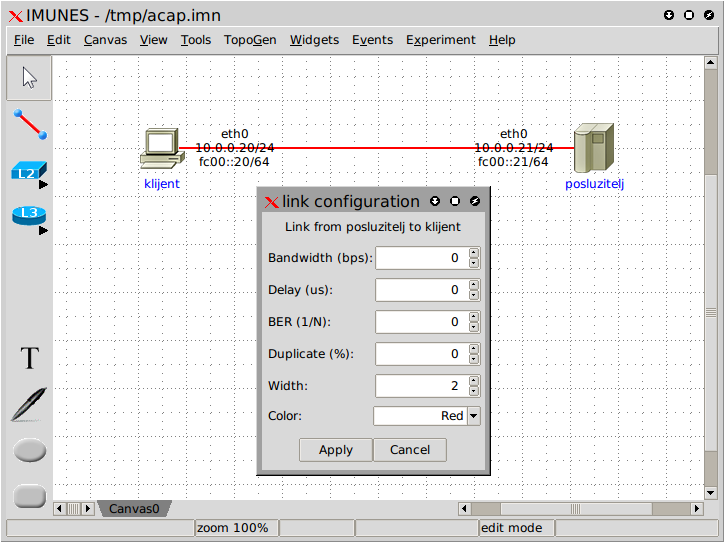
\includegraphics[width=0.82\textwidth]{imunes}
    \caption{Emulirana mrežna topologija za mjerenja u alatu IMUNES}
    \label{fig:imunes}
\end{figure}

Sva opisana mjerenja izvedena su na priloženoj topologiji uz promjenu
parametara na poveznici. Mjerenje kašnjenja izvedeno je u 50 iteracija
te je konačni prosjek prikazan pomoću grafikona i tablica.

\subsection{Utjecaj veličine javnih ključeva na veličinu poruka}

Duljina javnog ključa izravno utječe na veličinu digitalnog potpisa koji se
koristi za zaštitu poruka. S druge strane, duljina ključa povećava razinu
sigurnosti razmjene, ali ujedno i usporava računanje i verifikaciju digitalnih
potpisa. Kako se razvija i napreduje računalna moć tako se javlja potreba za sve
većom razinom sigurnosti. Na slici \ref{fig:key_size} prikazane su veličine
poruka za različite veličine RSA ključeva. Duljine poruka izražene su u
oktetima, dok su duljine ključeva prikazane na standardan način, u bitovima.
Može se zamijetiti kako
poruka \initi{} uopće ne ovisi o veličini javnog ključa jer ne sadrži niti javni
ključ niti digitalni potpis. Poruka \listr{} sadrži samo digitalni potpis, a
poruke \initr{} i \listi{} sadrže i digitalni potpis i javni ključ što je
vidljivo iz slike jer crte koje ih označuju najbrže rastu.

\begin{figure}[h]
    \centering
    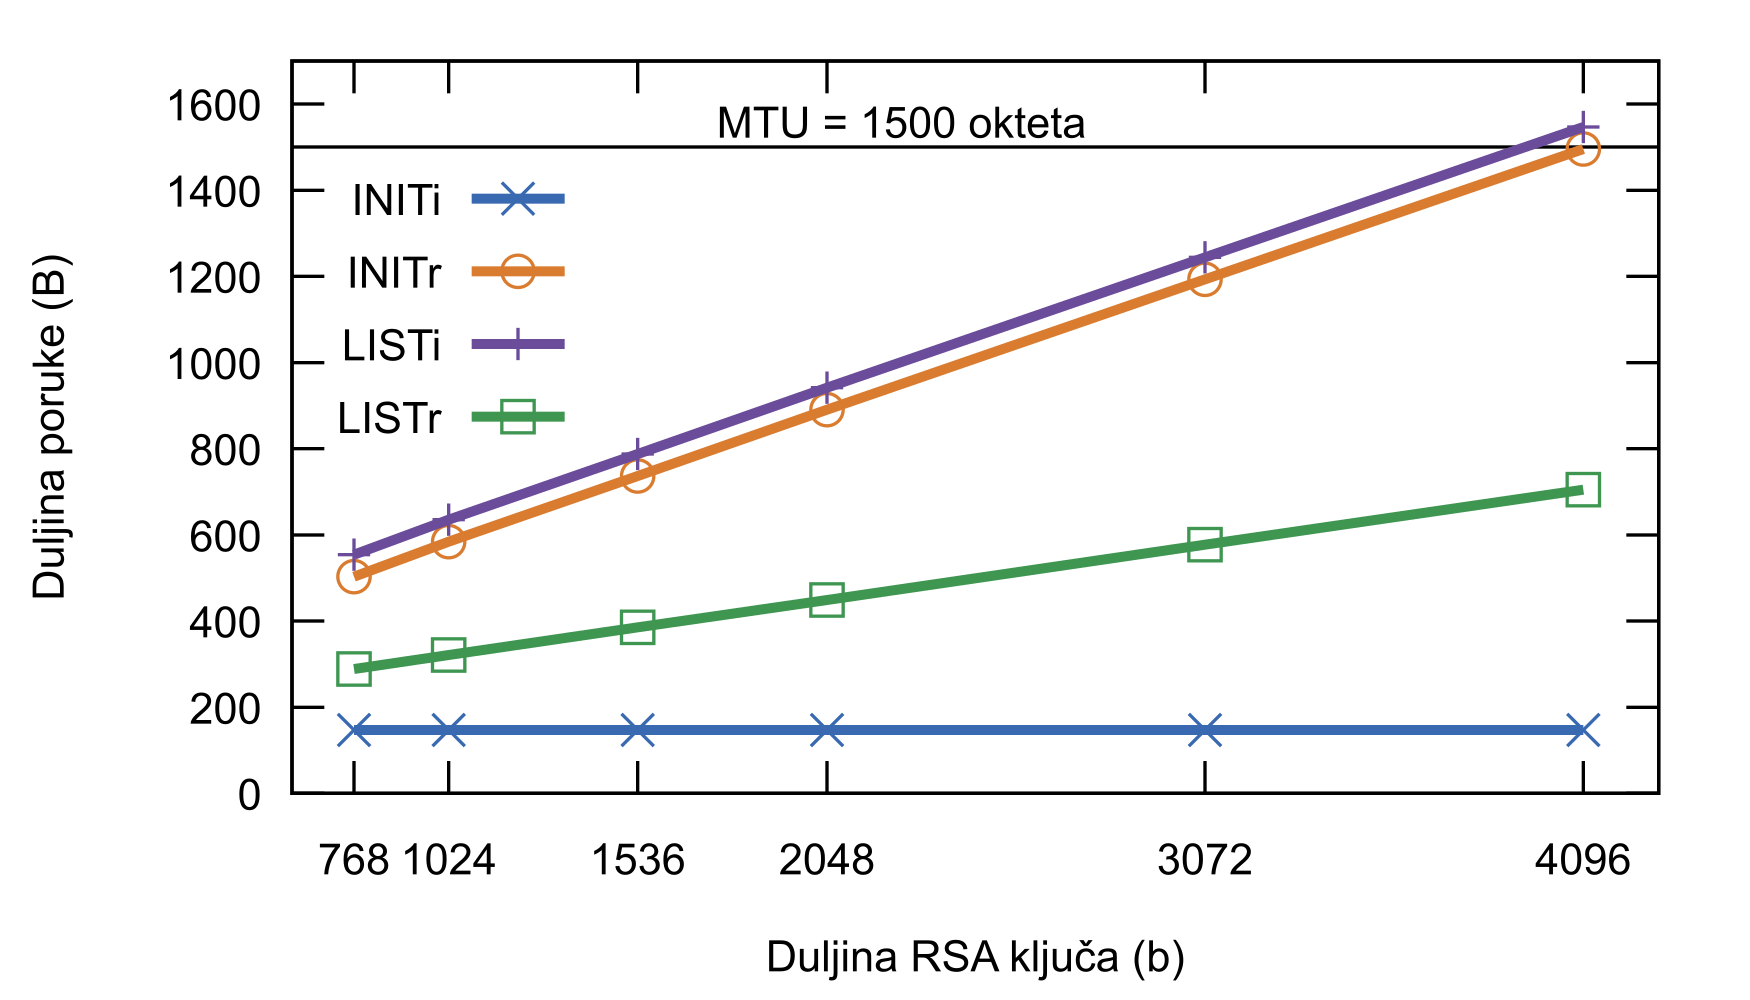
\includegraphics[width=0.7\textwidth]{key_size.png}
    \caption{Veličina poruka ovisno o veličini RSA javnih ključeva}
    \label{fig:key_size}
\end{figure}

Protokol Ethernet standardno podržava prijenos od najviše 1500 okteta podataka,
što je definirano najvećom jedinicom prijenosa (engl. \emph{Maximum
Transmission Unit} - MTU). Povećanje veličine RSA ključeva ili veliki popis podržanih
algoritama mogli bi onemogućiti korištenje protokola na sloju
Ethernet, odnosno zahtijevalo bi se
korištenje više poruka za razmjenu cijelog popisa, što nije predviđeno
specifikacijom i ostvarenjem protokola. Uz to, cilj je smanjiti veličinu
poruka kako bi se
povećala efikasnost i smanjila propusnost potrebna za razmjenu poruka i ubrzao
sam dogovor.

Smanjenje veličine poruka moguće je uvođenjem kriptografije koja se zasniva na
eliptičnim krivuljama i koristi manju veličinu javnih ključeva i digitalnih
potpisa. Mjerenja veličine poruka za različite veličine ECDSA ključeva
prikazana su na slici \ref{fig:key_size_ec}. 

\begin{figure}[h]
    \centering
    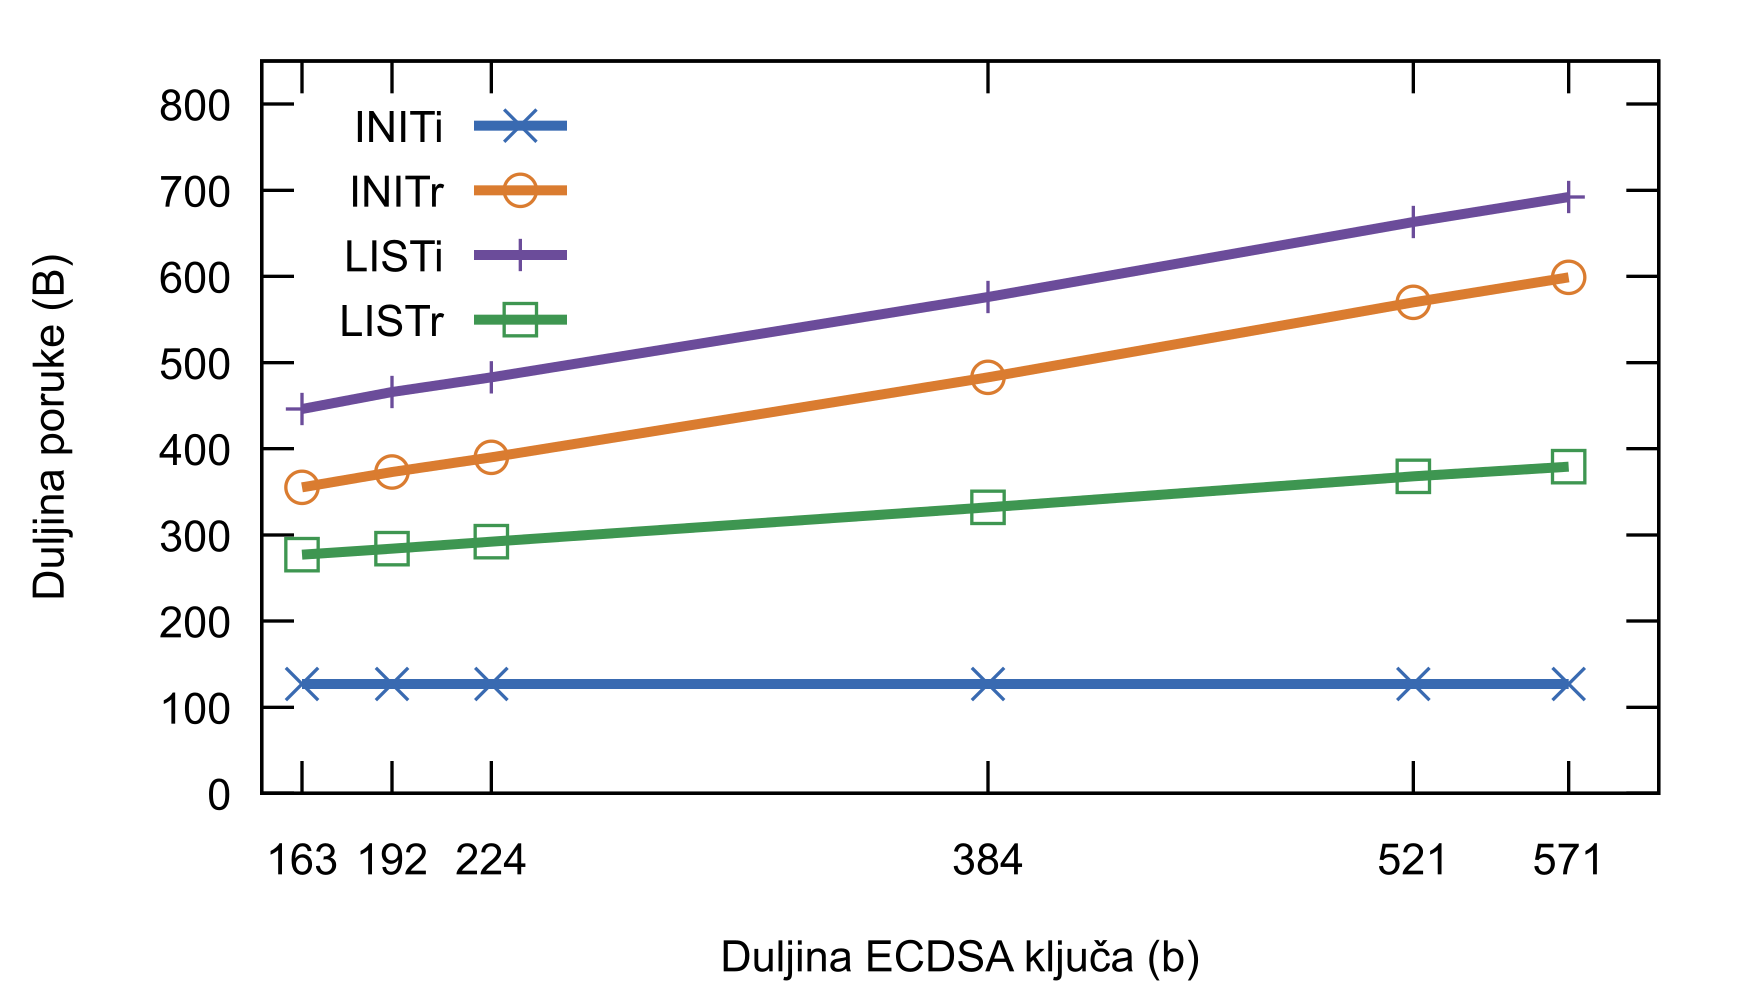
\includegraphics[width=0.7\textwidth]{key_size_ec.png}
    \caption{Veličina poruka ovisno o veličini ECDSA javnih ključeva}
    \label{fig:key_size_ec}
\end{figure}

Korištenjem ECDSA ključeva značajno se smanjuje veličina poruka protokola ACAP i
smanjuje potrebna propusnost za protokol. Važno je napomenuti da je
sigurnost koju pruža 224 bitni ECDSA ključ usporediva sa sigurnošću koju pruža
2048 bitni RSA ključ. Stoga, uvođenje kriptografije zasnovane na eliptičnim
krivuljama smanjuje potrebnu propusnost i ujedno povećava razinu sigurnosti.

\subsection{Trajanje dogovora ovisno o kašnjenju}

Trajanje dogovora mjereno je na strani klijenta tako da se jednosmjerno
kašnjenje mijenjalo od 0 ms sve do 400 ms, što predstavlja maksimalno kašnjenje
u oba smjera od 800 ms. Mjerenja su izvršena za sve transportne protokole, ali
razlike između protokola UDP, IPv4, IPv6 i Ethernet su premale i ne daju nikakav
dodatan uvid u mjerenja. Na slici \ref{fig:agreement_delay} prikazana su
mjerenja kašnjenja za protokole UDP, SCTP i TCP uz korištenje standardne
kriptografije i uz korištenje kriptografije zasnovane na eliptičkim krivuljama.

\begin{figure}[h]
    \centering
    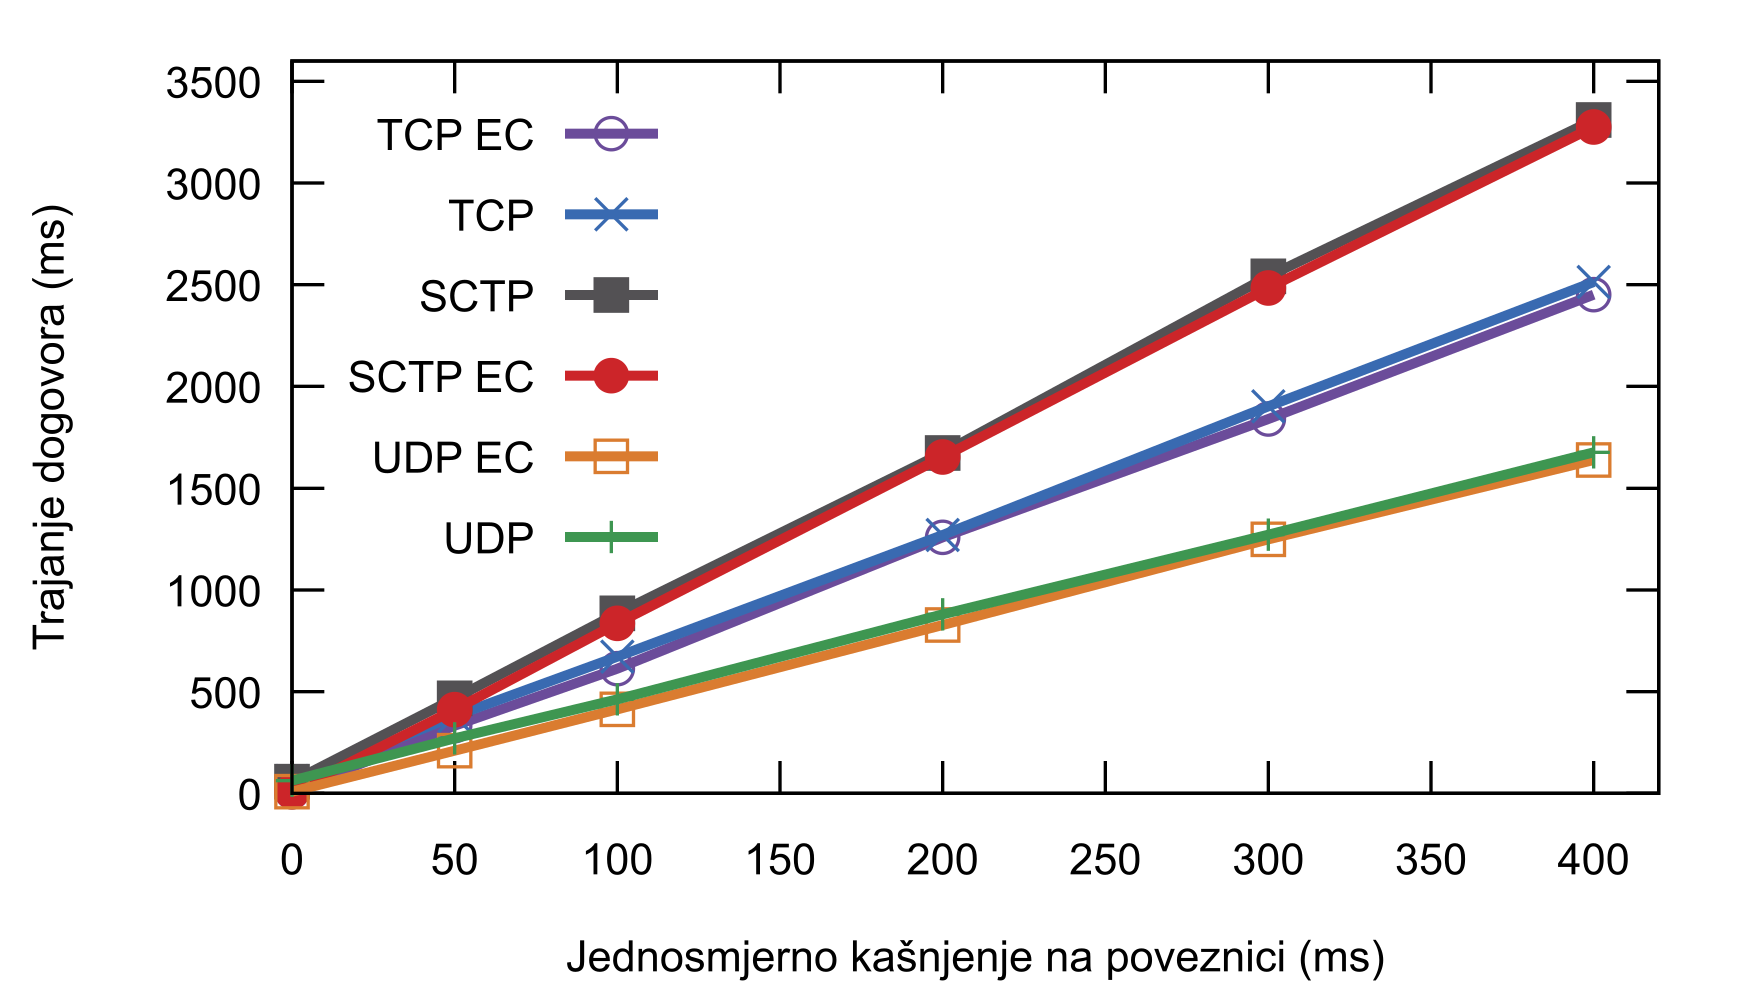
\includegraphics[width=0.7\textwidth]{agreement_delay2.png}
    \caption{Trajanje dogovora ovisno o kašnjenju, protokolu i korištenim algoritmima}
    \label{fig:agreement_delay}
\end{figure}

Prije svega, mogu se zamijetiti razlike između protokola UDP, SCTP i TCP koje su
ovisne o uspostavi veze kod tih protokola. UDP nema nikakve uspostave, protokolu
SCTP su potrebne 4 poruke, a protokolu TCP 3 poruke za uspostavu
veze. Slika \ref{fig:agreement_delay} ujedno pokazuje da je korištenje
eliptičnih krivulja manje zahtjevno, ali da i mala vrijednost kašnjenja
značajnije utječe na trajanje dogovora u odnosu na promjenu kriptografskih
operacija.

\subsection{Utjecaj propusnosti na trajanje dogovora}

Na slici \ref{fig:agreement_bw} prikazano je trajanje dogovora u odnosu na
brzinu u kilobitima u sekundi (Kbps). U mjerenja nisu uključeni rezultati za
više od 10 Mbps jer iznad te brzine nema razlike u trajanju dogovora. Protokol
ACAP ima
relativno male zahtjeve na propusnost jer se dogovor može dovršiti i na
poveznici brzine 10 Kbps ispod 2 sekunde.

\begin{figure}[h]
    \centering
    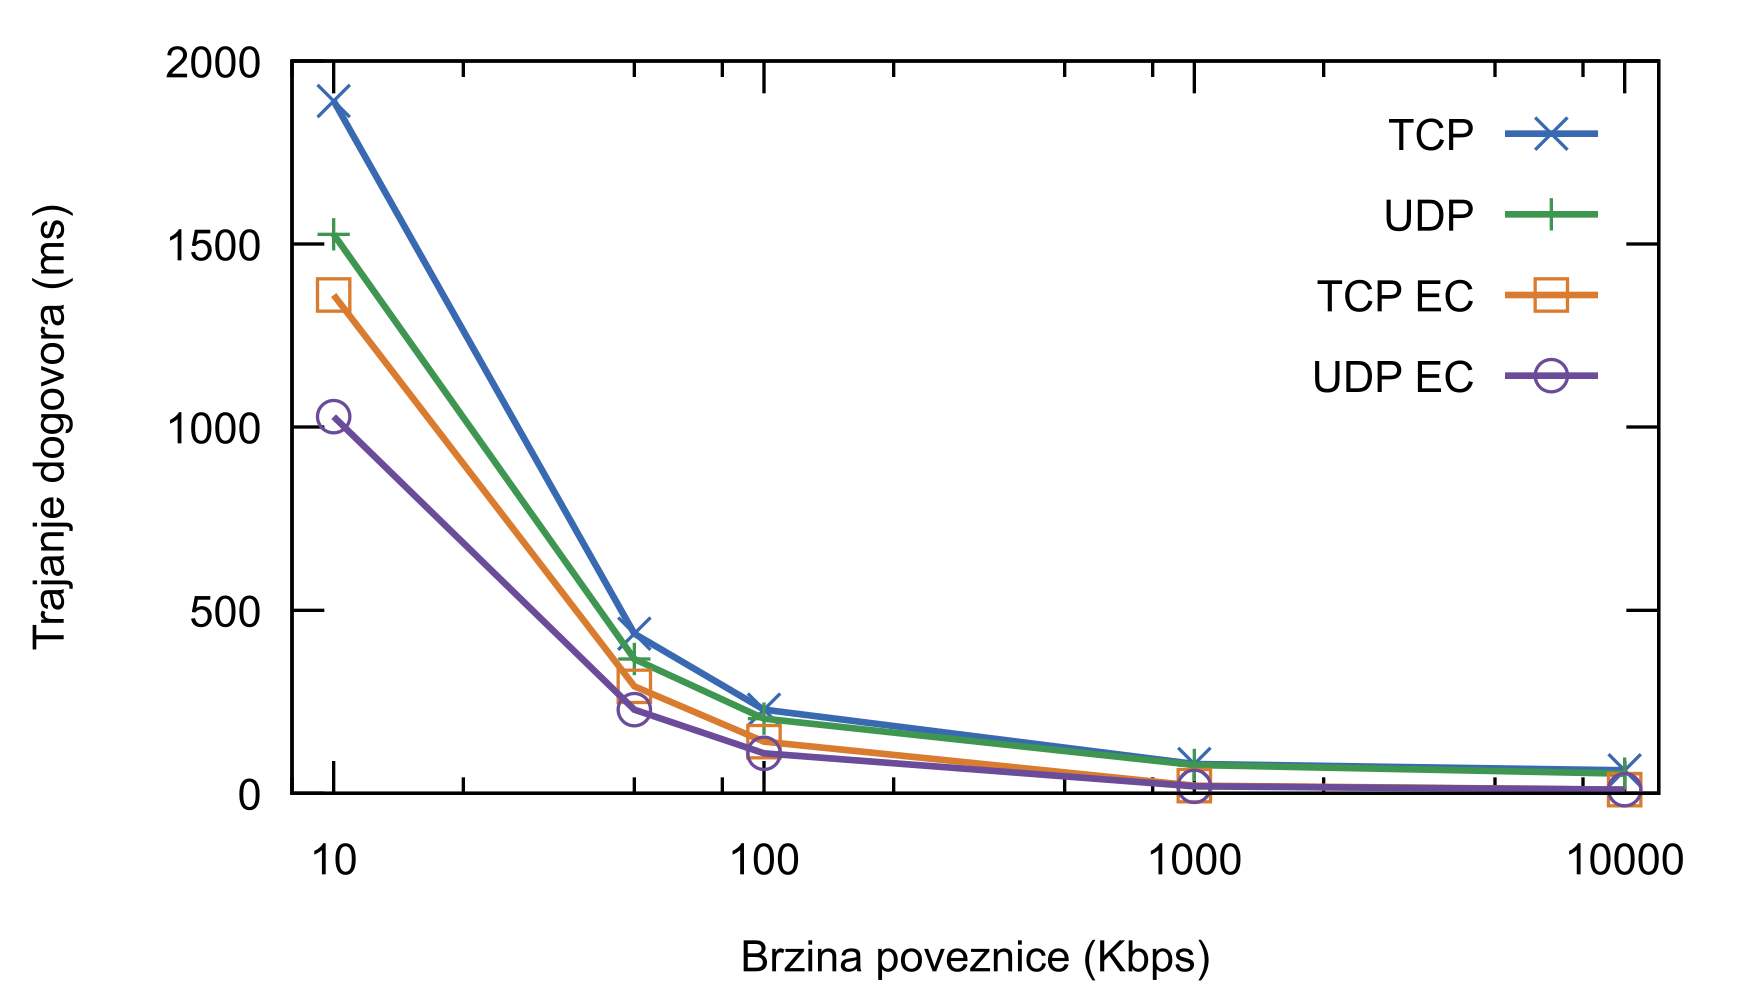
\includegraphics[width=0.7\textwidth]{agreement_bw.png}
    \caption{Trajanje dogovora ovisno o brzini poveznice, protokolu i korištenim algoritmima}
    \label{fig:agreement_bw}
\end{figure}

Uz korištenje kriptografije zasnovane na eliptičnim krivuljama dodatno se
smanjuju zahtjevi na propusnost poveznice, što ih čini osobito pogodnim za
dogovor na uređajima s ograničenim sposobnostima koji su prisutni u okolini
Interneta stvari.

Slika također pokazuje da je dodatan promet koji koriste standardni
kriptografski algoritmi u odnosu na EC algoritme veći od dodatnog prometa koji
generira signalizacija protokola TCP. U slučaju korištenja EC algoritama
dovoljno se ubrzava dogovor korištenjem protokola TCP, koji u tom slučaju postaje
valjana alternativa protokolu UDP i u uvjetima niske propusnosti.

\section{Složenost kriptografskih operacija u protokolu}
\label{sec:complex}

U protokolu ACAP izvode se sljedeće kriptografske operacije:
\begin{itemize}
    \item generiranje tajnog i javnog dijela za Diffie-Hellman razmjenu,
    \item računanje DH zajedničke tajne,
    \item računanje i provjera digitalnog potpisa i
    \item računanje i provjera HMAC zaštitne sume.
\end{itemize}

Trajanje stvaranja i obrade svake poruke u protokolu ACAP prikazano je u
tablici \ref{tab:obrada}. U tablici su vremena za stvaranje poruka označena
žutom bojom, dok su vremena obrade neoznačena. Mjerenja su rađena korištenjem standardnih
Diffie-Hellman parametara veličine 1536 bita te za ECDH korištenjem 163 bitne
eliptične krivulje koji pružaju usporedive razine sigurnosti. Za digitalni
potpis korišten je RSA-1536 kod standardnih algoritama, a ECDSA-sect163r2 kod EC
algoritama.

\begin{table}[htb]
\caption{Trajanje stvaranja i obrade poruka}
\renewcommand{\arraystretch}{1.3}
\label{tab:obrada}
\centering
\normalsize
\begin{tabular}{ l  r  r  r  r }
\toprule &
    Klijent &
    Poslužitelj &
    Klijent EC &
    Poslužitelj EC
    \\ \midrule
\initi{} &
    \colorbox{yellow!50}{47.207 ms} &
    \colorbox{white!50}{4.157 ms} &
    \colorbox{yellow!50}{1.483 ms} &
    \colorbox{white!50}{0.676 ms}
    \\ \hline
\initr{} &
    \colorbox{white!50}{4.284 ms} &
    \colorbox{yellow!50}{0.172 ms} &
    \colorbox{white!50}{1.125 ms} &
    \colorbox{yellow!50}{0.162 ms}
    \\ \hline
\listi{} &
    \colorbox{yellow!50}{0.365 ms} &
    \colorbox{white!50}{0.282 ms} &
    \colorbox{yellow!50}{0.432 ms} &
    \colorbox{white!50}{0.636 ms}
    \\ \hline
\listr{} &
    \colorbox{white!50}{0.171 ms} &
    \colorbox{yellow!50}{0.257 ms} & 
    \colorbox{white!50}{0.599 ms} &
    \colorbox{yellow!50}{0.342 ms}
    \\ \hline
Ukupno &
    52.009 ms &
    4.869 ms &
    3.460 ms &
    1.817 ms
    \\ \bottomrule
\end{tabular}
\end{table}

Za stvaranje poruke \initi{} potrebno je generirati tajni i javni dio za
Diffie-Hellman razmjenu na klijentskoj strani. To je računalno najzahtjevniji
dio cijelog dogovora i za standardne i za EC algoritme, što se odražava u
vremenima u tablici. Obrada poruke \initi{}
na poslužiteljskoj strani sastoji se od računanja Diffie-Hellman zajedničke
tajne, što predstavlja drugu najzahtjevniju operaciju u sklopu razmjene poruka.

Stvaranje poruke \initr{} uključuje izračun digitalnog potpisa i HMAC sažetka.
Izračun digitalnog potpisa kod poslužitelja odrađuje se u sklopu pozadinskog
procesa u svrhu smanjivanja utjecaj DoS napada na protokol ACAP, a izračun
HMAC-a može se odraditi tek po primitku poruke \initi{}. Obrada poruke
\initr{} sastoji se od provjere digitalnog potpisa i HMAC-a te računanja DH
zajedničke tajne. Dok su za standardne algoritme stvaranje i obrada \initr{}
slične zahtjevnosti, kod ECDSA algoritama složenost provjere digitalnog potpisa
veća je od složenosti računanja (za algoritam RSA vrijedi suprotno).

Stvaranje poruke \listi{} obuhvaća računanje digitalnog potpisa i HMAC zaštitne
sume koji se po primitku provjeravaju na strani poslužitelja. Posljednja poruka
\listr{} sadrži samo digitalni potpis koji se provjerava na strani klijenta
nakon primitka poruke. Kod ove poruke uočava se složenost stvaranja i
provjeravanja digitalnog potpisa kod standardnih i EC algoritama.

Ukupni rezultati mjerenja pokazuju kako je opterećenje veće na strani
klijenta u odnosu na poslužitelja, kod standardnih algoritama taj je odnos
veći nego kod EC algoritama zbog računalno zahtjevnog generiranja
dobrih Diffie-Hellman vrijednosti za zaštitu komunikacije. Razlika između
klijenta i poslužitelja postoji jer poslužitelj u pozadini generira DH
vrijednosti. Po potrebi bi se to moglo raditi i na klijentskoj strani kako bi se
smanjilo opterećenje kod početka dogovora.

\section{Dohvaćanje podržanih algoritama}

Dohvaćanje trenutno podržanih algoritama u sustavu izvedeno je pomoću vanjskog
alata koji generira listu u JSON formatu koja je kompatibilna s aktualnim
programskim ostvarenjem protokola ACAP. Rezultat izvođenja prikazan je na slici
\ref{fig:fetch_algs}. U danom primjeru algoritmi su raspoređeni po abecedi,
a konačan raspored uvjetovan je željenom razinom sigurnosti i ostalim
uvjetima okoline u kojoj se protokol izvodi. Primjerice, u uređaje se mogu
ugraditi prioriteti ili se oni mogu dohvaćati s nekog vanjskog servisa koji
će redovito rangirati kriptografske algoritme ovisno o duljini ključa ili izlaza i
postojećim napadima na te algoritme. Na raspoređivanje algoritama mogu
utjecati i različiti dokumenti i specifikacije vezani uz određenu
ustanovu, propisane standarde\footnote{Popis aktualnih standarda i preporuka
može se naći na: \url{http://www.keylength.com/}.} ili postupak certifikacije.

\begin{figure}[htb]
\begin{footnotesize}
\begin{verbatim}
{
  "algorithm types": {
    "hash": [
      "MD5", "RIPEMD160", "SHA1", "SHA224", "SHA256", "SHA384", "SHA512", "Whirlpool" ],
    "public_key": [
      "DSA_1024", "DSA_2048", "DSA_3072", "RSA_1024", "RSA_1536", "RSA_2048",
      "RSA_3072", "RSA_4096", "ECDSA_prime256v1_256", "ECDSA_sect163k1_163",
      "ECDSA_secp384r1_384", ... ],
    "secret_key": [
      "AES_ECB_128", "AES_CBC_128", "AES_CTR_128", "AES_ECB_192", "AES_CBC_192",
      "AES_CTR_192", "AES_ECB_256", "AES_CBC_256", "AES_CTR_256", "Blowfish_ECB_128",
      "Blowfish_CBC_128", ...  "Blowfish_CBC_152", "Blowfish_CTR_152", "CAST5_ECB_64",
      "CAST5_CBC_80", ...  "CAST5_ECB_112", "CAST5_CBC_112", "CAST5_CTR_112",
      "Camellia_ECB_128", "Camellia_CBC_128", ...  "Camellia_ECB_256", "Camellia_CBC_256",
      "Camellia_CTR_256", "IDEA_ECB_128", "IDEA_CBC_128", "IDEA_CTR_128", "SEED_ECB_128",
      "SEED_CBC_128", "SEED_CTR_128", "TripleDES_ECB_64", "TripleDES_CBC_64",
      "TripleDES_CTR_64", "TripleDES_ECB_128", "TripleDES_CBC_128", "TripleDES_CTR_128",
      "TripleDES_ECB_192", "TripleDES_CBC_192", "TripleDES_CTR_192" ]
  }
}
\end{verbatim}
\end{footnotesize}
\vspace{-20pt}
\caption{Skraćeni ispis alata za dohvaćanje podržanih kriptografskih algoritama}
\label{fig:fetch_algs}
\end{figure}

Trenutno podržani algoritmi ovise isključivo o biblioteci koja će se koristiti
za zaštitu komunikacije nakon dogovora algoritma, odnosno o vanjskoj aplikaciji
koja koristi protokol ACAP za dogovor svih preduvjeta potrebnih za zaštitu
komunikacije. U danom primjeru dohvaćaju se podržani algoritmi koje koristi
biblioteka \emph{cryptography} za Python 3 koja se radi brzine izvođenja oslanja
na biblioteku OpenSSL\footnote{https://www.openssl.org/}.

\section{Ostvareni sigurnosni mehanizmi}

Sigurnosni mehanizmi u protokolu ACAP uvedeni su na više različitih razina.
Osnovni mehanizmi izravno su vezani uz komunikacijski model te su opisani i
formalno verificirani kroz alat Scyther u poglavlju \ref{ch:verif}.
Ostatak sigurnosnih mehanizama izravno je vezan uz ostvarenje prototipa.
Ostvareni su sljedeći sigurnosni mehanizmi:
\begin{itemize}
    \item smanjenje utjecaja DoS napada iscrpljivanjem resursa na strani
	poslužitelja,
    \item sprječavanje napada ponavljanjem poruka,
    \item neovisnost kriptografskih ključeva za dogovor i ključeva za zaštitu
	komunikacije nakon dogovora.
\end{itemize}

Iz poglavlja \ref{sec:complex} vidljivo je da su najzahtjevnije operacije
vezane uz generiranje Diffie-Hellman vrijednosti i računanje DH tajnog ključa.
Na poslužiteljskoj strani bi se obje te operacije trebale odraditi po primitku
poruke \initi{}. Na taj način bi programsko ostvarenje bilo izravno izloženo
napadu gdje se generira veliki broj \initi{} poruka. Kako bi se spriječio taj
napad, generiranje DH vrijednosti odvojeno je u zasebnu proceduru koja
periodički u pozadini generira DH vrijednosti. Dodatno se uz generiranje vrijednosti
generira i digitalni potpis koji je sastavni dio poruke \initr{} ($S_R(g^r)$)
kako bi se smanjilo opterećenje stvaranja poruke \initr{}. U zadnjem redu
tablice \ref{tab:obrada} prikazane su ukupne vrijednosti obrade za klijenta i
poslužitelja. Te vrijednosti pokazuju da je trošak na strani mogućeg napadača,
odnosno klijenta, veći od troška na strani poslužitelja.

Napadač koji se nalazi na putu između poslužitelja i klijenta mogao bi spremiti
sve pakete uključene tijekom jedne razmjene i kasnije ponoviti cjelokupnu
razmjenu tako da se opet koriste prije dogovoreni ključevi i algoritmi.
Prvi dio obrane od takvog napada leži u osvježavanju DH vrijednosti na strani
poslužitelja, koja se generira svakih 30 sekundi. Novi javni dio DH razmjene
izravno će utjecati na ostatak razmjene te će provjere HMAC sažetka biti
neuspješne. Drugi dio obrane nalazi se u pamćenju prijašnjih \emph{nonce}
vrijednosti i odbijanju paketa s prethodno korištenim \emph{nonce}
vrijednostima.

Neovisnost kriptografskih ključeva postiže se uvođenjem pseudo nasumičnih
funkcija (engl. \emph{pseudo random function}, PRF) koje će iterativnim
korištenjem algoritma HMAC jamčiti računalnu neovisnost ključeva. Koncepti za
ostvarenje PRF-a preuzeti su iz protokola IKEv2~\cite{rfc5996} i jamče da
ključ koji se koristi za dogovor u protokolu ACAP neće otkriti nikakve podatke o
dijeljenom tajnom ključu koji je rezultat protokola ACAP.

% vim: spell spelllang=hr
